
\subsection{Mathmatical Model of a single Perceptron}	
		
A perceptron  a function that takes in several inputs and produces an output of either 0 or 1.\\ \\
The input of perceptron is usually modeled as a column vector. Let $X(n\times1)$ represent this column vector. The perceptron applies weights to each values in the $X$ and then sums them together \cite{book}. In other words, the perceptron finds a linear combination of the matrix $X$ as show below.
$$
X = 
\begin{bmatrix}
	x_1 \\
	x_2 \\
	x_3 \\
	\vdots \\
	x_n
\end{bmatrix} 
$$
Let $\alpha$ be a possible linear combination of $X$. 
$$
	\alpha = \sum_{i=1}^{n} a_ix_i = a_1x_1 + a_2x_2 + \dots + a_nx_n
$$
At first, the $a_i$ are chosen randomly. However, during the training process they will be adjusted until they are able to produce the optimal output \cite{book}. \\ \\
The next step of the perceptron utilizes an activation function. An activation function can be either 0 or 1, depending on a threshold value. The threshold value is selected based on the specific use of the perceptron \cite{book}. Below is an example of an activation function. Let $T$ represent the threshold value.

$$f(x) = 
	\begin{array}{cc}
  	\{ & 
    \begin{array}{cc}
    	1 & x >= T \\
    	0 & x < T
    \end{array}
\end{array}
$$
The output of the perceptron is the output of the activation function above(since this is a single layer perceptron).

\subsection{Layering perceptrons}

Perceptrons gain a lot more functionality when they are used in combination with other perceptrons. Let $p_i$ represent a perceptron. Perceptrons are stacked together to build column vectors of perceptrons as show below.

$$
	P = \begin{bmatrix}
		p_1 \\
		p_2 \\
		\vdots \\
		p_3
	\end{bmatrix}
$$
A column vector of perceptrons is called a layer. There are three kinds of perceptron layers. There is an input layer. The input layer is always the first layer in any multilayered perceptron. Then, there is the output layer. This layer is always the last layer, and as the name suggests this is the output of the multilayer perceptron. In between the output layer and the input layer are the hidden layers. There can be any number of hidden layers in a perceptron. Each of these layers use the output of the layer right before it as its input.

\begin{center}
	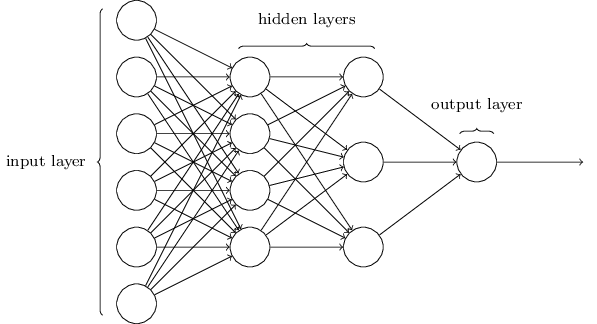
\includegraphics[scale=0.5]{multilayer-perceptron2}
\end{center}
\cite{image1}
The diagram aboves represents how a multilayer perceptron is structured. Notice how each perceptron takes in all the outputs from the layer before it. This multilayer perceptron only has 1 output, however, it is possible to structure a perceptron to output multiple values if needed. An example of a multilayer perceptron with multiple outputs is shown below.

\begin{center}
	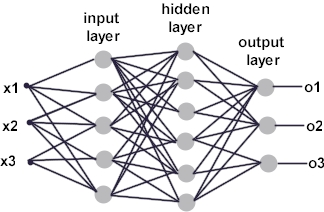
\includegraphics[scale=0.5]{multilayer-perceptron}
\end{center}
\cite{image2}
The structure above is used when the problem is more complex. For example, a perceptron that takes in the pixel values of an image of a handwritten number and then outputs what it thinks the number is needs 10 outputs, 1 for each possible value. \\ \\
A perceptron can be a very useful tool for difficult problems such as recognizing handwriting, because they can be used to build any possible logical function. Designing multilayered perceptrons to read handwriting is significantly easier than trying to write the explicit logical statements for it.

\subsection{Training}

\subsubsection{Sigmoid Neuron}

A perceptron as currently described is not very useful if you are trying to train a multilayer perceptron to work as intended. For this purpose we replace the perceptrons we have been currently using with the more powerful sigmoid neurons. A sigmoid neuron works very similarly to the standard perceptron. However, the key difference is that unlike a perceptron a sigmoid neuron can output any value between 0 and 1 \cite{book}. Additionally, the method in which the output of the neuron is computed is different than the computation for the standard perceptron. Let column vector $A$ represent the input for the sigmoid neuron.

$$
	A = 
	\begin{bmatrix}
		a_1 \\
		a_2 \\
		\vdots \\
		a_n
	\end{bmatrix}
$$

\begin{center}
	let $Z = \sum_{i=1}^{n} w_ia_i - b$
\end{center}
where $b$ is a bias and $w_i$ is the weight being applied to the ith input. The bias is utilized instead of using the threshold as was used before with standard perceptron. Let $W=[w_i]$ so that $Z$ can be written as

$$	W=
	 \begin{bmatrix}
		w_1 & w_2 & \dots & w_n
	\end{bmatrix}
$$
$$	
	Z = \begin{bmatrix}
		w_1 & w_2 & \dots & w_n
	\end{bmatrix}	
	\bullet
	\begin{bmatrix}
		a_1 \\ a_2 \\ \vdots \\ a_n	
	\end{bmatrix} - b
	 = W \bullet A - b
$$
The sigmoid function $$\sigma(Z) = \frac{1}{1+e^{-Z}}$$ is used to take any input and return a value between 0 and 1 \cite{book}. This is useful because the value of $Z$ is not constrained to $[0, 1]$. However, we need the output to be $\in [0, 1]$ for analysis and the next layer of perceptrons. \\ \\
The sigmoid neuron is useful because it always the training algorithm to make small adjustments to the weights and biases, which in turn allows us to make small adjustments to the output of the multilayered perceptrons \cite{book}. Training is quite difficult without using sigmoid neurons because the values are binary. Thus, we cannot comprehend the impact of a small change to the output. 

\subsubsection{Cost Function}
The Cost function is a formula that takes the perceptron output and the correct output as the input and outputs how bad or good the multilayer perceptron is \cite{book}. The training algorithm uses the cost function to determine what effects changes on the weights and biases have on the accuracy of the multilayered perceptron.\\ \\

Let 
$$
	A = \begin{bmatrix}
		a_{11} & a_{12} & \dots & a_{1m} \\
		a_{21} & a_{22} & \dots & a_{2m} \\
		\vdots \\
		a_{n1} & a_{n2} & \dots & a_{nm}
	\end{bmatrix}
	C = \begin{bmatrix}
		c_{11} & c_{12} & \dots & c_{1m} \\
		c_{21} & c_{22} & \dots & c_{2m} \\
		\vdots \\
		c_{n1} & c_{n2} & \dots & c_{nm}
	\end{bmatrix}
$$
Where the column vectors of $A$ represent the desired output of the multilayered perceptron, and where the column vectors of $C$ represent the actual output of the multilayered perceptron. If $C(w, b)$ is the cost function, then

$$
	C(w, b) = \frac{1}{2n} \sum_{i=1}^{m} ||(A^T)_i-(C^T)_i||^2
$$
Where $w$ and $b$ represent the weights and biases that are needed to compute $C$.

\subsubsection{Gradient Descent}

Gradient descent is the algorithm that is used to improve the multilayered perceptron. The purpose of gradient descent is to minimize the cost function. This is because the accuracy of the multilayered perceptron is better when the cost function is closer to 0 \cite{book}. \\ \\
Gradient descent achieves this goal by computing the negative gradient of the cost function.

$$
	g(a) = -\nabla C(w,b)
$$
The function $g(a)$ points in the direction in which the Cost function is decreasing the fastest, we know this to be true because $\nabla C(w,b)$ points in the direction the cost function increase the fastest by the definition of the gradient. The process by which the gradient of the cost function is computed is called backpropagation and is beyond the scope of this paper.\\ \\
The $g(a)$ function is used to find the direction in which the all the weights and biases need to be modified to minimize the cost function. Once a small modification to the weights and biases are made $g(a)$ is recalculated and the weights and baises are changed again. This process continues until we find a local minimum of the cost function.\\ \\
Gradient descent occurs in n dimensional space, where n is the number of weights and biases that the multilayered perceptron has. There are usually thousands of weights and biases in a multilayered perceptron. Because of this, it very difficult to visualize the process of gradient descent. However, it is possible to visualize a much simpler example in $R^3$.

\begin{center}
	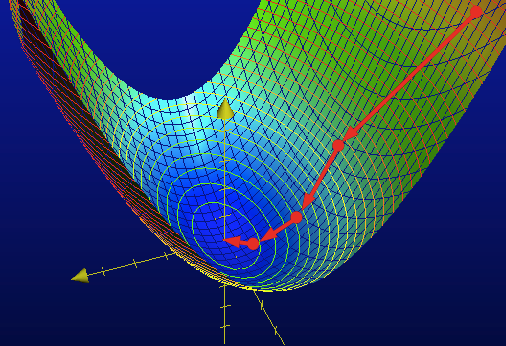
\includegraphics[scale=0.5]{images/gradientdescent}
\end{center}
\cite{image3}
It is clear from the diagram above, that the gradient descent algorithm moves the cost function closer and closer towards a local minimum.\\ \\
It should be reemphasized that this is local minimum, not a global minimum. This means that gradient descent does not necessarily give you the best answer. The task of finding a global minimum of the cost function is a much harder task to accomplish. Overall, the gradient descent algorithm is the most efficient method of finding a local minimum of the cost function. This can be proven using the Cauchy-Schwarz inequality \cite{book}. This is left as an exercise for the reader. 
